%---
\section{\DSp}
\label{sec:proto}

%({\it giuliana.fiorlillo@na.infn.it})  \\


With \DSps\ the \DS\ Collaboration aims at constructing and operating a prototype detector of intermediate size (\DSpApproximateMass) , incorporating the new \DSks\ technologies for their integration and full validation.  

%The choice of the \DSpApproximateMass\ mass scale allows for a full validation of the technological choices for DarkSide-20k. 

The prototype will evolve to include elements of the detectors soon as they are available and inter-faceable to the rest of the chain.  In some cases, preliminary elements will be gradually replaced by final ones as soon as available.  Radiopure materials will be used for the prototype whenever the time scale of the project and readiness of the corresponding screening activities allow.

Thus, \DSps\  is not intended to replace validation and tests made in laboratories, but rather complement them with the integration with the rest of the detector.  The prompt execution of \DSps\ is crucial to fulfil the overall schedule of \DSks.  \DSps\ is on the critical path of the project.

The program for DarkSide-Proto is expected to span over three different phases:

\begin{compactenum}
\item Test of cryogenic system concept at test site; identification and preparation of full readout and \DAQ\ of 50 pre-production PDMs (two Motherboards); 
\item Design, construction and assembly at test site of cryostat and \LArTPC\ equipped with 50 preproduction \DSkPdms; assembly, commissioning, and operation of full read-out and DAQ for 50 \DSkPdms;
\item Assembly and commissioning of full system, including 400 first production PDMs; full readout and DAQ operational; evolution towards final configuration. 
\end{compactenum}

The plan for DarkSide-Proto was reviewed, approved, and funded by the CNS2 of INFN. Requests for funding from other participating groups are being evaluated or will be submitted in the near future. 

In August 2017 the DS Collaboration and LNGS reached and finalized an agreement \cite{Mapelli:2017vn} with the Accelerator \& Technology Sector of CERN and its Technical Division to construct and commission the DS-20k cryogenics at CERN, with support from the Cryogenics Group and the Vacuum, Surfaces and Coatings Group (both groups are part of CERN's Technical Division). The extension of this program to carry out the first surface operation of DarkSide-Proto at CERN before moving the detector to LNGS was agreed by the CERN Accelerator \& Technology Sector via an Addendum to the above agreement. The necessary space and facilities are the same as for the test on the DarkSide-20k cryogenics and are already allocated.

A radio-pure 1ton cryostat for DarkSide-Proto was built by Tecno Alarm, s.r.l., Roma, and delivered at CERN in August 2018 (see Fig.\ref{fig:proto-cern}).
The 1 mBq/kg U/Th AISI 304 L Steel was procured from NIRONIT Edelstahlhandel GmbH \& Co and it is good enough to be used for a possible physics run in LNGS and described in section \ref{sec:DSl}.

\begin{figure}[h!]
\centering
\includegraphics[width=\columnwidth]{./Figures/proto-cern.png}
\caption{The \DSp\ cryostat  delivered  at CERN}
\label{fig:proto-cern}
\end{figure}

Assembly and test of the DS-20k cryogenics will take place at CERN, during the last quarter of 2018 and first quarter of 2019. Construction of DS-Proto is expected in 2019. A first test operation with a reduced number of photosensors is expected by the end of 2018, followed by a second operation with a full complement of PDMs in 2019.

Full characterization of the prototype performance and physics runs will be performed after installation at LNGS. The detailed program of the activities to be carried out underground is under study.

We anticipate that, since the DarkSide-Proto will be a stand alone system, sharing the DarkSide-20k cryogenics system at LNGS will not be possible. However over the past few years of R\&D for the DarkSide-20k cryogenics, we have realized and tested several key components which will be more than capable of handling the prototype system. These parts can be used for DarkSide-Proto with minor system integration together with most of the DarkSide-50 and existing R\&D devices.

%\subsection{Technical specifications}
%The DS-20k cryogenics and gas handling system consists of several subsystems: 1) a cryostat hosting the LAr TPC, 2) a gas handling system including heat exchanger and argon condenser, 3) a purification system consisting of a hot getter and a cold synthetic charcoal radon trap, 4) a LAr handling system including the recovery units with their own gas handling systems and cold liquid transfer lines, 5) a LN2  plant providing a cooling source on reserve, and 6) cryogenic shipping vessels for delivery of UAr. 
%
%The key features of the DS-20k cryogenics and gas handling system are:
%\begin{itemize}
%\item Ability to efficiently cool down and purify 50 t of UAr at the $< $ 0.1 ppb purity level (O$_2$  content equivalent), which guarantees a $>$5 ms electron lifetime, while maintaining a stable pressure in the detector (within 0.1 psi);
%\item Ability to obtain a total gas recirculation flow equivalent to 1000 std L/min, which permits us to reach the desired purity of LAr during the course of about one month. This is driven by two custom made high-fow-rate gas pumps, mirroring the design principles and strategy of DS-50, with upgraded sizing of all components. The notable difference with respect to DarkSide-50 is the addition of a fast liquid withdrawal loop, connected to the bottom of the cryostat through a custom designed bayonet assembly that also allows for fast draining of the detector in case of unexpected problems;
%\item Usage of new high efficiency heat exchangers to recover cooling power during fast purification circulation, exploiting a new custom-designed argon condenser with variable cooling power (from 0kW to 5kW). Heat exchangers boil off LAr that is drawn out of the bottom of the cryostat and at the same time cool the GAr coming from the hot getter as it heads towards the radon trap first, and then the condenser;
%\item Wide cooling power range to cover fast initial argon filling as well as normal operations, and TPC-off mode. With efficient thermal management, the total external cooling power needed to maintain the system in TPC-off mode is about 150W;
%\item Incorporation of the robust safety features based on the experience with DS-50, including a feature that keeps the system immune from total failure of the main LNGS power line, by the use of a local UPS unit and a local LN2  storage system. The backup system can work for 3 days off a small LN2  reservoir located on the top of the condenser and for as long as $> 30$ days off the central LN2  storage.
%\end{itemize}
%
\subsection{The DarkSide-Proto TPC}

The TPC mechanics, including the structural elements, the field cage, the reflector cage, the transparent cathode, the transparent anode (also serving as a diving bell for the containment of the gaseous phase), the SiPM assemblies, the high-voltage feed system, will all be built utilising, on a scaled down overall dimension, the same design and construction techniques foreseen for the baseline of DarkSide-20k. 

The photodetector modules will be arranged to cover the top and bottom of the TPC. Both top and bottom planes consist of 185 photodetector modules assembled into 5 SQBs and 4 TRBs. As described in section \ref{sec:DAQ}, the readout chain will evolve from commercial components used in the first phase allowing full digitisation of pulse shape, towards the planned final components as they become available at each stage of the development. Also optical signal transmission, once and if available, can be tested on a significant number of channels. 

The DarkSide-Proto photosensors are arranged in 18 Motherboards made of 25 (SQB) or 15 (TRB) PDMSs, requiring 370 SiPM tiles. Bonding $\sim$ 9,000 SiPMs in few months is one of the most demanding tasks of this detector. The NOA facility will not be operative before summer 2019, while the Proto schedule foresees a delivery of the 18 Motherboards by July 2019.

The production of the SiPMs by the LFoundry company requires a technological transfer from the FBK company. The time schedule agreed between the two companies foresees the delivery of the first SiPMs by the end of February 2019.

The time window available to bond the 370 tiles stays therefore between the devil and the deep blue: on one side the SiPMs will not be available before February 2019 while on the other side the NOA personnel have to start their equipment learning by fall 2019, that includes periods spent in the company headquarters.

The construction strategy relies on two bonding facilities, the first one located at Princeton University and the second one at LNGS. According to the experience gained in the past months, a bonding rate of 3 tiles/day is feasible: we need therefore 60 working days, corresponding to 12 weeks (3 months), to bond the 370 tiles  in the two facilities.

The man power at LNGS can be provided by the NOA contracts, while finding man power at Princeton University is more challenging. Different options were evaluated, and others are under consideration. 
The University of Manchester (UK) has identified a candidate who will
spend a significant amount of time in the course of the next year to be
trained.
%The Manchester University (UK) showed an interest to join the Princeton facility effort and they are starting their procedure to select a candidate. 

A tight connection between the two production sites has to be provided, to include the harmonization of the procedures and quality assurance test. A link person is being identified.

LNGS requires a significant increase of man power: after the bonding the tiles will be equipped with a Front End Board (FEB), mounted and tested ad LNGS. After the assembly the tiles and the FEB will be tested in LN.  The first Motherboard, made of 25 PDMs, was just assembled .
The Motherboard will be shipped to Napoli, where a comprehensive test at cryogenic temperature is scheduled.

A powerful test facility has to be prepared at Napoli, requiring extra man power. The procedures and the tools to ship the Motherboard from Pisa to Napoli and from Napoli to CERN have to be carefully planned and made available. 

\subsection{Materials for DarkSide-Proto}

DS-Proto is a test bench of DS-20k. It won't be used to demonstrate the material radio-purity requirements of DS-20k, however It will be built with the goal of achieving the best radio-purity conceivable at the time of the construction, based on the current results of materials assay campaign. Additionally, DS-Proto can be used to assess the possible contamination related to the detector construction procedures (TPC/PE), evidencing material cleaning/handling issues.

The assessment of the DS-Proto radioactive budget will be obtained through the material assay campaign and the Monte Carlo simulation. The validation of the predictions concerning the neutron/gamma originated by the material contamination will be only possible through a data taking underground with DS-Proto deployed in a proper shielding. A physics run, focused on the low WIMP mass search, will be eventually possible with the S2-only analysis in the keV region. In this context, the minimizations of the low-energy gamma background of the prototype will be extremely important.


\subsection{Validation tests and operation}
Upon successful completion of the test phase of the different parts, we plan to measure the overall performance of the DarkSide-Proto through some key parameters: the S1 light yield, the drift, electro-luminescence field and gas pocket thickness uniformity for high resolution of S2 signals and the $x y$ position reconstruction. 

To the purpose of optimizing the S2 signals, the first two Motherboards will be assembled into a small TPC with reduced size drift length to avoid pile-up (see Fig.\ref{fig:mini-proto}). 
This set-up will allow for early studies of the S2 formation and readout, to be carried out while the pre-production of the remaining Motherboards of the prototype is ongoing.

Full test of the S1 response and therefore of the SiPM readout chain can be obtained at surface by switching off the electroluminescence field. 
%It is very likely that due to the cosmic ray flux at surface, to test S2 we need to run the detector underground. 
\begin{figure}[h!]
\centering
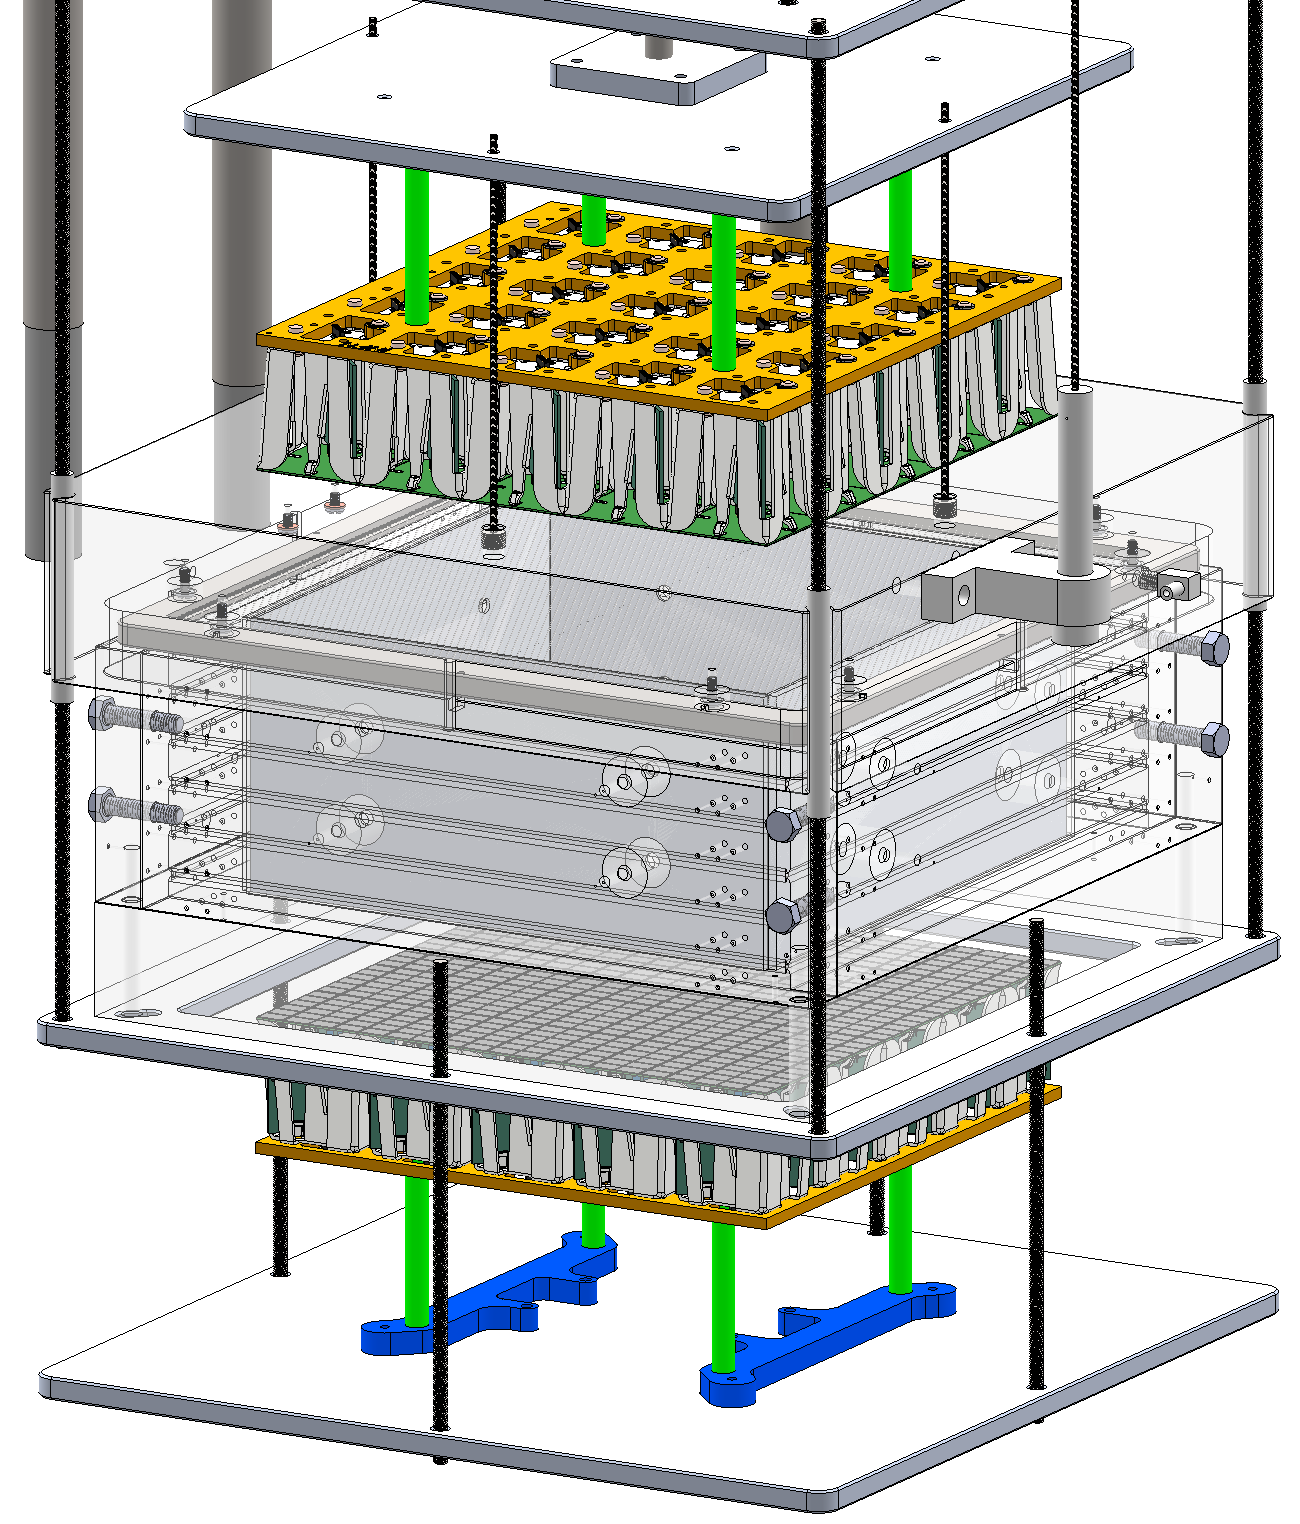
\includegraphics[width=\columnwidth]{./Figures/mini-proto.png}
\caption{Schematics   of  the setup for the optimization of  the S2 signals}
\label{fig:mini-proto}
\end{figure}